%%%%%%%%%%%%%%%%%%%%%%%%%%%%%%%%%%%%%%%%%
% Focus Beamer Presentation
% LaTeX Template
% Version 1.0 (8/8/18)
%
% This template has been downloaded from:
% http://www.LaTeXTemplates.com
%
% Original author:
% Pasquale Africa (https://github.com/elauksap/focus-beamertheme) with modifications by 
% Vel (vel@LaTeXTemplates.com)
%
% Template license:
% GNU GPL v3.0 License
%
% Important note:
% The bibliography/references need to be compiled with bibtex.
%
%%%%%%%%%%%%%%%%%%%%%%%%%%%%%%%%%%%%%%%%%

%----------------------------------------------------------------------------------------
%	PACKAGES AND OTHER DOCUMENT CONFIGURATIONS
%----------------------------------------------------------------------------------------

\documentclass{beamer}


\usepackage{amssymb}
\usepackage{amsmath}
%\usepackage{enumitem}
%\newcommand{\checkeditem}{\item[\refstepcounter{enumi}$\text{\rlap{$\checkmark$}}\square$]}

\newcommand{\dichajos}{\vec{\Delta}}
\newcommand{\cychajos}{\overset{\circ}{\Delta}}


\usepackage{pgf,tikz}
\usetikzlibrary{arrows}
\usetikzlibrary{decorations.markings}


\usetheme{focus} % Use the Focus theme supplied with the template
% Add option [numbering=none] to disable the footer progress bar
% Add option [numbering=fullbar] to show the footer progress bar as always full with a slide count

% Uncomment to enable the ice-blue theme
%\definecolor{main}{RGB}{92, 138, 168}
%\definecolor{background}{RGB}{240, 247, 255}

%------------------------------------------------

\usepackage{booktabs} % Required for better table rules

%\footskip 2cm
%\evensidemargin 0pt
%\oddsidemargin 0pt

%%%%%%%%%%%%%%%%%%%%%%%%%%%%%%%% FONTS 
\usepackage[utf8]{inputenc}
\usepackage[T1]{fontenc}
\usepackage{times}

\usepackage{xspace}
%%%%%%%%%%%%%%%%%%%%%%%%%%%%%%%% HEADER
%\usepackage{fancyhdr}
% \pagestyle{headings}
%%\fancyhf{}
%%\fancyhead[LE,RO]{ \chaptername\ \thechapter \chaptermark}
%%\fancyhead[RE,LO]{Guides and tutorials}
%%\fancyfoot[CE,CO]{\leftmark}
%%\fancyfoot[LE,RO]{\thepage}






%%%%%%%%%%%%%%%%%%%%%%%%%%%%%%%% MATHS
\usepackage{longtable}
\usepackage{amsmath,amsthm,amssymb,amsthm}
\usepackage{enumerate}

%%%%%%%%%%%%%%%%%%%%%%%%%%%%%%%% ALGORITHMS
\usepackage{algorithm}
\usepackage{algpseudocode}
\algnewcommand\algorithmicinput{\textbf{Input:}}
\algnewcommand\algorithmicoutput{\textbf{Output:}}
\algnewcommand\Input{\item[\algorithmicinput]}
\algnewcommand\Output{\item[\algorithmicoutput]}
\renewcommand{\algorithmicforall}{\textbf{for each}}

%%%%%%%%%%%%%%%%%%%%%%%%%%%%%%%% HYPERREFS
\usepackage{hyperref}%\usepackage{url}

%%%%%%%%%%%%%%%%%%%%%%%%%%%%%%%% FIGURES
\usepackage{caption}
\usepackage{subfigure}
\usepackage{tikz}
\usepackage{svg}

\usepackage{pdftricks}
%\usepackage[pdf]{pstricks}
\begin{psinputs}
	\usepackage{pstricks,pst-plot,pst-node,pst-func}
\end{psinputs}
%\PassOptionsToPackage{pdf}{pstricks} %used for pdflatex
%\usepackage{auto-pst-pdf}
\usepackage{graphics,graphicx}

%Drawings
%\usepackage{tkz-graph}
\tikzstyle{vertex}=[circle, draw, inner sep=0pt, minimum size=6pt]
\newcommand{\vertex}{\node[vertex]}

%----------------------------------------------
% MARGES

%Index et marges
 \usepackage{marginnote}
% \renewcommand*{\marginfont}{}

%mots de l'index dans la marge ou pas
\newcommand{\m}[1]{}
%\newcommand{\m}[1]{\marginnote[\raggedright{\textit{\scriptsize #1}}]{\raggedleft{\textit{\scriptsize #1}}}}

\newcommand{\g}[1]{{\em #1}}
\newcommand{\mg}[1]{\g{#1}\m{#1}}
\newcommand{\ig}[1]{\g{#1}\index{#1}}
\newcommand{\mi}[1]{\m{#1}\index{#1}}
\newcommand{\mig}[1]{\mg{#1}\index{#1}}

%%% empasize + index %%%
 %\let\oldmarginpar\marginpar
 %\renewcommand\marginpar[1]{\-\oldmarginpar [\raggedright{\small #1}]{\raggedleft{\small #1}}}
 



%%%%%%%%%%%%%%%%%%%%%%%%%%%%%%%% THEOREMS
%\usepackage[framemethod=tikz]{mdframed}
%
%\mdfdefinestyle{mystyle}{
%  hidealllines=true,
%  leftline=true,
%  innerleftmargin=10pt,
%  innerrightmargin=10pt,
%  innertopmargin=-9pt,
%  innerbottommargin=1pt,
%}
%
%\surroundwithmdframed[style=mystyle]{definition}
%\surroundwithmdframed[style=mystyle]{theorem}


\usepackage{amsthm}
\usepackage{thmtools}



%\theoremstyle{plain}
%\newtheorem{theorem}{Theorem}[section]
%\newtheorem{proposition}[theorem]{Proposition}
%\newtheorem{property}{Property}[theorem]
%\newtheorem{assert}{Assertion}[theorem]
%\newtheorem*{assertnonum}{Assertion}
%\newtheorem{corollary}[theorem]{Corollary}
%\newtheorem{lemma}[theorem]{Lemma}
%\newtheorem{obs}[theorem]{Observation}
%
%\theoremstyle{definition}
%\newtheorem{definition}[theorem]{Definition}
%\newtheorem{exercise}{Exercise}[section]
%\newtheorem{problem}[theorem]{Problem}
%\newtheorem{conjecture}[theorem]{Conjecture}
%\newtheorem{algorithm}[theorem]{Algorithm}
%
%\theoremstyle{remark}
%\newtheorem{remark}[theorem]{Remark}
%\newtheorem{example}[theorem]{Example}
%\newtheorem{claim}{Claim}[theorem]


%(dirchi paper)
\newenvironment{subproof}{\par\noindent {\it Proof}.\ }{\hfill$\lozenge$\par\vspace{11pt}}


%%%%%%%%%%%%%%%%%%%%%%%%%%%%%%%% 
% 			MACROS				          %%%%%%%%
%%%%%%%%%%%%%%%%%%%%%%%%%%%%%%%%



\newcommand{\Gya}{Gy\'arf\'as\xspace}
\newcommand{\Sze}{Szemerédi\xspace}
\newcommand{\Erd}{Erd\H os\xspace}
\newcommand{\Rod}{R\"{o}dl\xspace}
\newcommand{\Chu}{Chudnovsky\xspace}
\newcommand{\Kur}{Kuratovski\xspace}
\newcommand{\Vus}{Vu\v{s}kovi\'c\xspace}
\newcommand{\Haj}{Hajnal\xspace}
\newcommand{\Lov}{Lov\'asz\xspace}
\newcommand{\Kra}{Kr\'al\xspace}
\newcommand{\Krato}{Kratochvil\xspace}
\newcommand{\Kam}{Kaminski\xspace}
\newcommand{\Gro}{Gr\"otschel\xspace}
\newcommand{\Hag}{H\"aggkvist\xspace}

\newcommand{\tred}[1]{\textcolor{red}{#1}}

%%%  Macros Maths %%%

\newcommand{\eN}{\mathbb{N}}
\newcommand{\bfN}{\mathbf{N}}
\newcommand{\eR}{\mathbb{R}}
\newcommand{\bfR}{\mathbf{R}}
%\newcommand{\bfZ}{\mathbf{Z}}
%\newcommand{\bfQ}{\mathbf{Q}}
%\newcommand{\bfC}{\mathbf{C}}

\newcommand{\mcal}[1]{\mathcal{#1}}
\newcommand{\sm}{\setminus}
\newcommand{\mc}{\mathcal}

\newcommand{\mF}{\mathcal{F}}
\newcommand{\mT}{\mathcal{T}}
\newcommand{\mB}{\mathcal{B}}
\newcommand{\mC}{\mathcal{C}}
\newcommand{\mP}{\mathcal{P}} 
\newcommand{\mM}{\mathcal{M}} 
\newcommand{\mV}{\mathcal{V}} 
\newcommand{\mA}{\mathcal{A}}
\newcommand{\mH}{\mathcal{H}}
\newcommand{\mU}{\mathcal{U}}


%%% Arrows %%%
\newcommand{\ra}{\rightarrow}
\newcommand{\Ra}{\Rightarrow}
\newcommand{\la}{\leftarrow}
\newcommand{\La}{\Leftarrow}
\newcommand{\orla}[1]{\overleftrightarrow{#1}}
\newcommand{\ora}[1]{\overrightarrow{#1}}
\newcommand{\ova}[1]{\overline{#1}}
\newcommand{\ovlra}{\overleftrightarrow}

\newcommand{\rs}{\rightsquigarrow}

%%% Graphs %%%

\DeclareMathOperator{\chr}{\chi}
\DeclareMathOperator{\ome}{\omega}
\DeclareMathOperator{\alp}{\alpha}
\DeclareMathOperator{\girth}{girth}
\DeclareMathOperator{\tw}{\mathrm{tw}}
\DeclareMathOperator{\tri}{\chi_T}
\DeclareMathOperator{\dic}{\ora \chi}

\DeclareMathOperator{\Forb}{Forb}
%\newcommand{\F}[1]{\Forb_{ind}{#1}}
\newcommand{\F}[1]{\Forb{#1}}
\newcommand{\dF}[1]{\ora{Forb{#1}}}

\DeclareMathOperator{\lexlabel}{label}
\DeclareMathOperator{\lcm}{lcm}
\DeclareMathOperator{\LexCycle}{LexCycle}
\DeclareMathOperator{\LexBFS}{LexBFS}



\newcommand{\Ct}{\ora{C_{3}}}
\newcommand{\TTt}{\ora{TT_{3}}}
\newcommand{\dichr}{\ora{\chr}}

\DeclareMathOperator{\trans}{tt}
\DeclareMathOperator{\Or}{Or}
\DeclareMathOperator{\Reach}{Reach}

%----------------------------------------------------------------------------------------
%	 TITLE SLIDE
%----------------------------------------------------------------------------------------

\title{Decomposition theorem for \\ locally out-transitive tournaments}

\subtitle{\small{Joint work with Pierre Charbit and Pierre Aboulker}}

\author{Guillaume Aubian}

%\titlegraphic{\includegraphics[scale=0.5]{Images/logo_ulm.png}} % Optional title page image, comment this line to remove it

\institute{TALGO/IRIF}

\date{18 june 2021}

%------------------------------------------------



\begin{document}


\tikzset{->-/.style={decoration={
  markings,
  mark=at position .5 with {\arrow{>}}},postaction={decorate}}}



%------------------------------------------------

\begin{frame}
	\maketitle % Automatically created using the information in the commands above
\end{frame}

%----------------------------------------------------------------------------------------
%	 SECTION 1
%----------------------------------------------------------------------------------------


\begin{frame}{dichromatic number}


            \centering

	    \begin{definition}
	            $G = (V,E)$ $k$-colourable iff $V = \bigcup\limits_{i=1}^{k} V_{i}$
 and $G[V_{i}]$ are acyclic.
	    \end{definition}



            \begin{tikzpicture}[line cap=round,line join=round,>=triangle 45, scale=3]
            \draw [->-] (-0.62,0.32) -- (0.13,0.5);
            \draw [->-] (0.13,0.5) to[bend left = 13] (-0.11,-0.24);
            \draw [->-] (-0.11,-0.24) -- (0.49,-0.12);
            \draw [->-] (0.49,-0.12) -- (0.13,0.5);
            \draw [->-] (-0.11,-0.24) to[bend left = 13] (0.13,0.5);
            \begin{scriptsize}
            \fill[red] (-0.62,0.32) circle (1pt);
            \fill[blue] (0.13,0.5) circle (1pt);
            \fill[red] (-0.11,-0.24) circle (1pt);
            \fill[red] (0.49,-0.12) circle (1pt);
            \end{scriptsize}
            \end{tikzpicture}
            $$\dic(G) = \min_{k} \{ k | G\text{ }k\text{-colourable} \} = 2$$
            $$\dic( \mathcal{G}) = \max \{ \dic(G) | G \in \mathcal{G} \}$$
\end{frame}

\begin{frame}{Induced subgraphs}
    \centering
	\begin{tikzpicture}[line cap=round,line join=round,>=triangle 45, scale=1.7]

        \begin{scope}[xshift=0cm,yshift=0.5cm]
            \draw [->-](-0.62,0.32)-- (0.13,0.5);
            \draw [->-](0.13,0.5)-- (-0.11,-0.24);
            %\draw [->-](-0.11,-0.24)-- (0.49,-0.12);
            %\draw [->-](0.49,-0.12) -- (0.13,0.5);
            \node at (1,0) {$\subseteq_{ind}$};
            \begin{scriptsize}
            \fill (-0.62,0.32) circle (1pt);
            \fill (0.13,0.5) circle (1pt);
            \fill (-0.11,-0.24) circle (1pt);
            %\fill (0.49,-0.12) circle (1pt);
            \end{scriptsize}
        \end{scope}

        \begin{scope}[xshift=0cm,yshift=-0.5cm]
            \draw [->-](-0.62,0.32)-- (0.13,0.5);
            \draw [->-](0.13,0.5)-- (-0.11,-0.24);
            \draw [->-](-0.11,-0.24)-- (0.49,-0.12);
            %\draw [->-](0.49,-0.12) -- (0.13,0.5);
            \node at (1,0) {$\not\subseteq_{ind}$};
            \begin{scriptsize}
            \fill (-0.62,0.32) circle (1pt);
            \fill (0.13,0.5) circle (1pt);
            \fill (-0.11,-0.24) circle (1pt);
            \fill (0.49,-0.12) circle (1pt);
            \end{scriptsize}
        \end{scope}

        \begin{scope}[xshift=3cm,scale=2]
            \draw [->-](-0.62,0.32)-- (0.13,0.5);
            \draw [->-](0.13,0.5)-- (-0.11,-0.24);
            \draw [->-](-0.11,-0.24)-- (0.49,-0.12);
            \draw [->-](0.49,-0.12) -- (0.13,0.5);
            \begin{scriptsize}
            \fill (-0.62,0.32) circle (1pt);
            \fill (0.13,0.5) circle (1pt);
            \fill (-0.11,-0.24) circle (1pt);
            \fill (0.49,-0.12) circle (1pt);
            \end{scriptsize}
        \end{scope}

	\end{tikzpicture}

    $$\F{(\mathcal{G})} = \{ H | \forall G \in \mathcal{G}, G \not\subseteq_{ind} H \}$$

\end{frame}

\begin{frame}{Some classes of digraphs}
    \centering
    \begin{itemize}
        \item Oriented graphs : $\F{(K_{2})}$
        \item Tournaments : $\F{(K_{2},K_{2})}$
        \item $TT_{k}$ : $\F{(K_{2},K_{2},C_{3})}$
        \item Hero : $H$ such that $\dic(\F{(K_{2},K_{2},C_{3})})$ bounded
    \end{itemize}
\end{frame}

\begin{frame}{The conjecture}
        \begin{block}{Conjecture (Aboulker, Charbit, Naserasr, 2020)}
        $H$ hero, $F$ oriented forest

        $\dic(\F{K_{2},H,F})$ bounded if and only if:

        \begin{itemize}
            \item $F$ is the disjoint union of stars or
            \item $H$ is transitive
        \end{itemize}
        \end{block}

    \only<2>{$$H \in \{ K_1 , K_2 \}, F \in \{ K_1 , K_2 \} \rightarrow \text{Trivial}$$}
%\end{frame}




%\begin{frame}{Special case we are interested in}

\only<3> {

Thus, easiest remaining case :

    \hspace{1cm}

    \centering

	\begin{tikzpicture}[line cap=round,line join=round,>=triangle 45, scale=2]

        \begin{scope}[xshift=0cm]
            \draw [->-](0.13,0.5) -- (-0.62,0.32) ;
            \draw [->-](0.13,0.5)-- (-0.11,-0.24);
            %\draw [->-](-0.11,-0.24)-- (0.49,-0.12);
            %\draw [->-](0.49,-0.12) -- (0.13,0.5);
            \begin{scriptsize}
            \fill (-0.62,0.32) circle (1pt);
            \fill (0.13,0.5) circle (1pt);
            \fill (-0.11,-0.24) circle (1pt);
            %\fill (0.49,-0.12) circle (1pt);
            \end{scriptsize}
        \end{scope}

        \begin{scope}[xshift=1.5cm]
            %\draw [->-](-0.62,0.32)-- (0.13,0.5);
            \draw [->-](0.13,0.5)-- (-0.11,-0.24);
            \draw [->-](-0.11,-0.24)-- (0.49,-0.12);
            \draw [->-](0.49,-0.12) -- (0.13,0.5);
            \begin{scriptsize}
            %\fill (-0.62,0.32) circle (1pt);
            \fill (0.13,0.5) circle (1pt);
            \fill (-0.11,-0.24) circle (1pt);
            \fill (0.49,-0.12) circle (1pt);
            \end{scriptsize}
        \end{scope}

	\end{tikzpicture}
}

\end{frame}

\begin{frame}{Our result}

    \begin{theorem}
        $\dic(\F{(K_2,K_{1,2},W_4)}) \leq 2$
    \end{theorem}

    \hspace{1cm}

    \centering

	\begin{tikzpicture}[line cap=round,line join=round,>=triangle 45, scale=2]

        \begin{scope}[xshift=0cm]
            \draw [->-](-0.62,0.32) -- (0.13,0.5);
            \draw [->-](-0.62,0.32) -- (-0.11,-0.24);
            \draw [->-](-0.62,0.32) -- (0.49,-0.12);
            \draw [->-](0.13,0.5)-- (-0.11,-0.24);
            \draw [->-](-0.11,-0.24)-- (0.49,-0.12);
            \draw [->-](0.49,-0.12) -- (0.13,0.5);
            \node at (0,0.7) {$W_4$};
            \begin{scriptsize}
            \fill (-0.62,0.32) circle (1pt);
            \fill (0.13,0.5) circle (1pt);
            \fill (-0.11,-0.24) circle (1pt);
            \fill (0.49,-0.12) circle (1pt);
            \end{scriptsize}
        \end{scope}

        \begin{scope}[xshift=1.5cm]
            \draw [->-](0.13,0.5) -- (-0.62,0.32) ;
            \draw [->-](0.13,0.5)-- (-0.11,-0.24);
            %\draw [->-](-0.11,-0.24)-- (0.49,-0.12);
            %\draw [->-](0.49,-0.12) -- (0.13,0.5);
            \node at (0,0.7) {$K_{1,2}$};
            \begin{scriptsize}
            \fill (-0.62,0.32) circle (1pt);
            \fill (0.13,0.5) circle (1pt);
            \fill (-0.11,-0.24) circle (1pt);
            %\fill (0.49,-0.12) circle (1pt);
            \end{scriptsize}
        \end{scope}


	\end{tikzpicture}


\end{frame}

\begin{frame}{locally out-transitive}
\begin{itemize}
    \item $\F{(\{W_4\})}$ $\rightarrow$ out-neighbourhood triangle-free
    \item $\F{(\{K_{1,2}\})}$ $\rightarrow$ out-neighbourhood semicomplete
\end{itemize}

Thus $\F{(\{K_2,W_4,K_{1,2}\})}$ $\rightarrow$ out-neighbourhood transitive

We call these \emph{locally out-transitive}
\end{frame}

\begin{frame}{Proof structure}
\begin{enumerate}
    \item Decomposition theorem for $\F{(K_2,W_4,K_{1,2})}$
    \item \begin{itemize}
            \item Use this to prove $\dic(\F{(K_2,K_{1,2},W_4)}) \leq 2$
            \item Prove Caccetta-\Hag for $\F{(K_2,K_{1,2},W_4)}$
          \end{itemize}
\end{enumerate}

These results are thus implied for $\F{(K_2,K_{1,2},C_3)}$
\end{frame}

\begin{frame}{in-round oriented graphs}
\begin{definition}
An oriented graph $D=(V,A)$ is in-round if there exists a cyclic order of $V$ such that :

$$\forall xy\in A, \forall z\in ]x,y[, zy\in A$$
\end{definition}

\centering

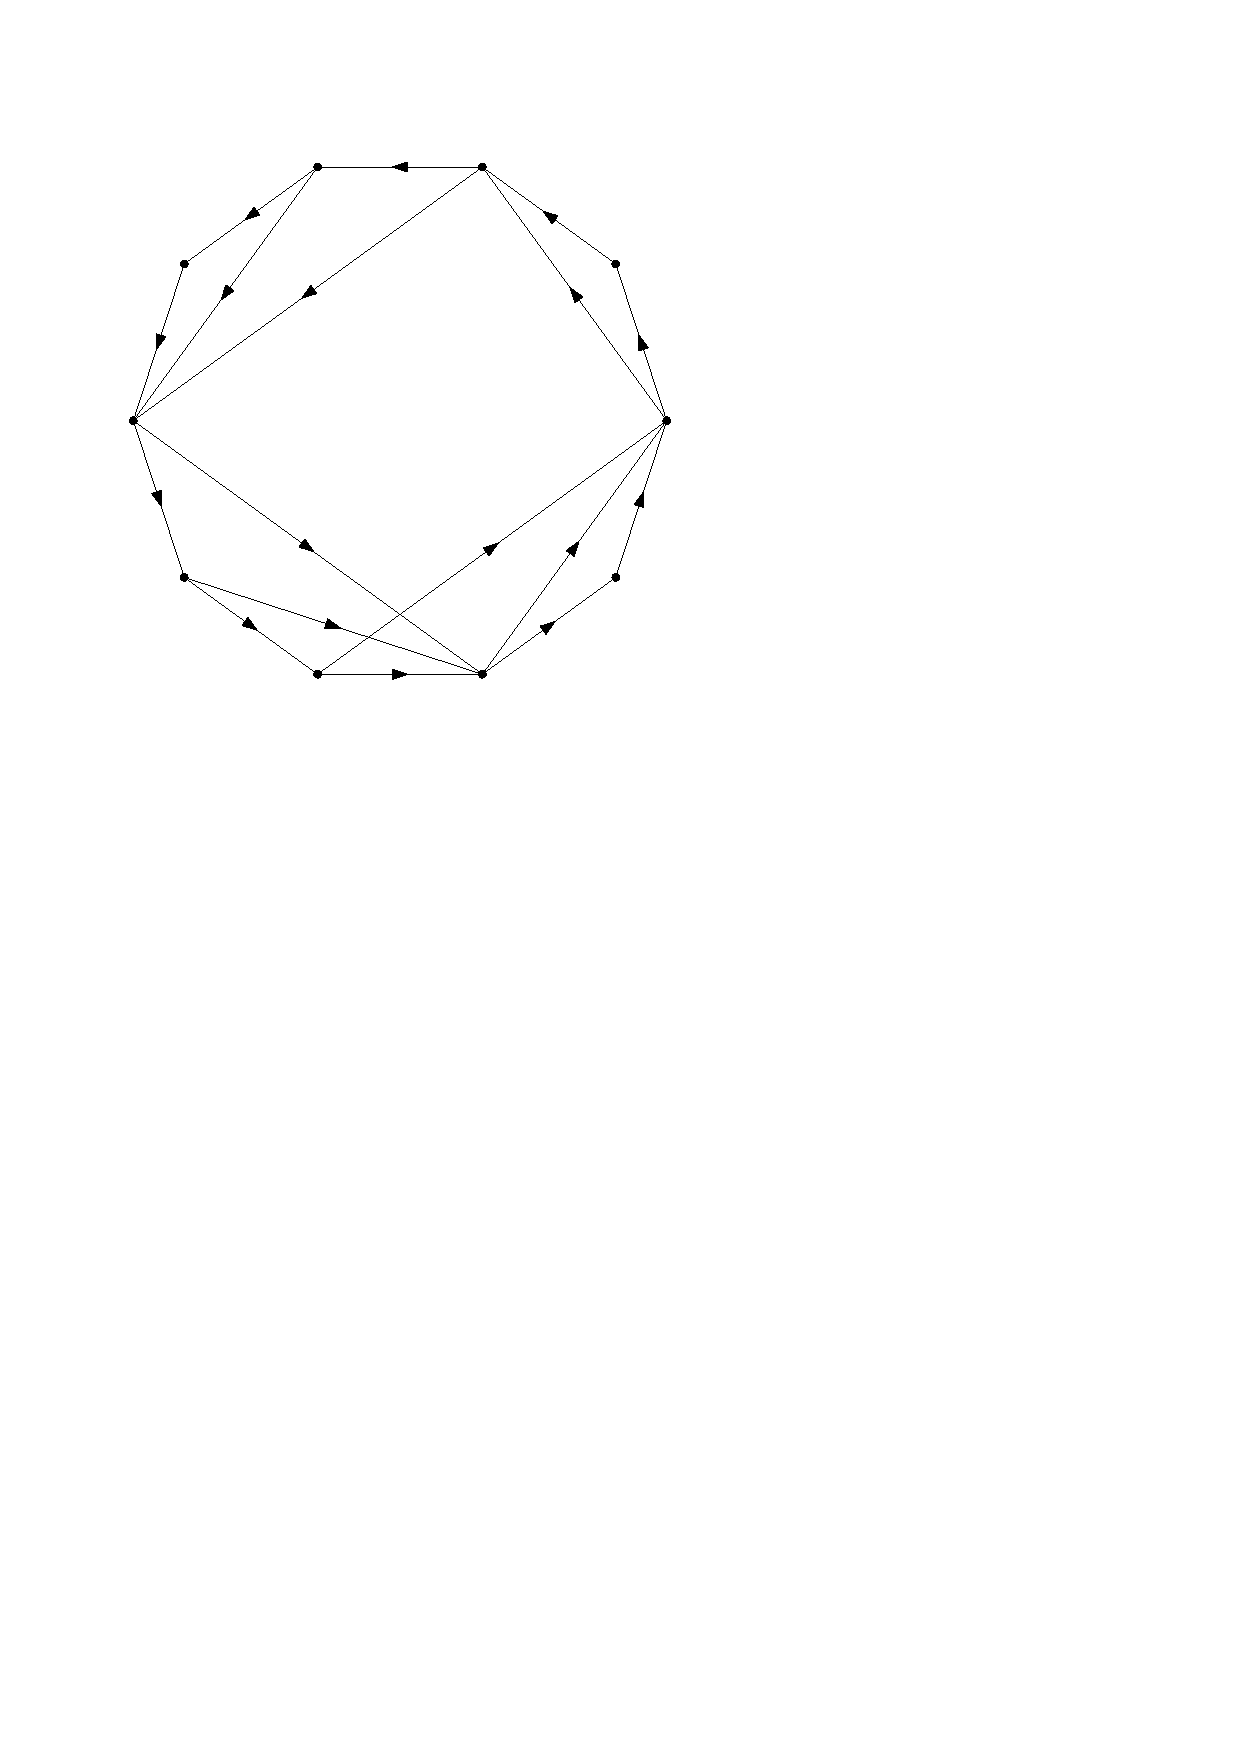
\includegraphics[scale=0.5]{Images/inround.pdf}
\end{frame}

\begin{frame}{in-round theorem}
\begin{theorem}
Let $D$ be a strong oriented graph such that for every vertex $x$, $x^+$ induces a tournament and $x^-$ induces an acyclic digraph. Then $D$ is in-round.
\end{theorem}

\pause

\textbf{Proof :}

\centering
	\begin{tikzpicture}[line cap=round,line join=round,>=triangle 45, scale=2]

        \begin{scope}
            \draw [->-] (0.13,0.5) -- (-0.62,0.32);
            \draw [->-] (-0.11,-0.24) -- (-0.62,0.32);
            \draw [->-,red] (0.49,-0.12) --(-0.62,0.32);
            \draw [->-] (0.13,0.5)-- (-0.11,-0.24);
            \draw [->-] (-0.11,-0.24)-- (0.49,-0.12);
            \draw [->-] (0.13,0.5) -- (0.49,-0.12);
            \begin{scriptsize}
            \fill[red] (-0.62,0.32) circle (1pt);
            \fill (0.13,0.5) circle (1pt);
            \fill (-0.11,-0.24) circle (1pt);
            \fill (0.49,-0.12) circle (1pt);
            \end{scriptsize}
        \end{scope}
    \end{tikzpicture}
\end{frame}

\begin{frame}{In-round theorem proof}

    \centering

    \only<1>{

	\begin{tikzpicture}[line cap=round,line join=round,>=triangle 45, scale=2]
        \begin{scope}
            \draw [->-] (-1,0) -- (0,2);
            \draw [->-,red] (-2,-1) -- (-1,0);
            \draw [->-,red] (-1,0) -- (1,0);
            \draw [->-,red] (1,0) --(2,-1);
            \begin{scriptsize}
            \fill (0,2) circle (1pt);
            \fill (-1,0) circle (1pt);
            \fill (1,0) circle (1pt);
            \fill (-2,-1) circle (1pt);
            \fill (2,-1) circle (1pt);
            \end{scriptsize}
        \end{scope}
    \end{tikzpicture}
    }

    \only<2>{

	\begin{tikzpicture}[line cap=round,line join=round,>=triangle 45, scale=2]
        \begin{scope}
            \draw [->-] (-1,0) -- (0,2);
            \draw [dashed] (1,0) -- (0,2);
            \draw [->-,red] (-2,-1) -- (-1,0);
            \draw [->-,red] (-1,0) -- (1,0);
            \draw [->-,red] (1,0) --(2,-1);
            \begin{scriptsize}
            \fill (0,2) circle (1pt);
            \fill (-1,0) circle (1pt);
            \fill (1,0) circle (1pt);
            \fill (-2,-1) circle (1pt);
            \fill (2,-1) circle (1pt);
            \end{scriptsize}
        \end{scope}
    \end{tikzpicture}
    }

    \only<3>{

	\begin{tikzpicture}[line cap=round,line join=round,>=triangle 45, scale=2]
        \begin{scope}
            \draw [->-] (-1,0) -- (0,2);
            \draw [->-,blue] (1,0) -- (0,2);
            \draw [->-,red] (-2,-1) -- (-1,0);
            \draw [->-,red] (-1,0) -- (1,0);
            \draw [->-,red] (1,0) --(2,-1);
            \begin{scriptsize}
            \fill (0,2) circle (1pt);
            \fill (-1,0) circle (1pt);
            \fill (1,0) circle (1pt);
            \fill (-2,-1) circle (1pt);
            \fill (2,-1) circle (1pt);
            \end{scriptsize}
        \end{scope}
    \end{tikzpicture}
    }

    \only<4>{

	\begin{tikzpicture}[line cap=round,line join=round,>=triangle 45, scale=2]
        \begin{scope}
            \draw [->-] (-1,0) -- (0,2);
            \draw [->-,blue] (0,2) -- (1,0);
            \draw [->-,red] (-2,-1) -- (-1,0);
            \draw [->-,red] (-1,0) -- (1,0);
            \draw [->-,red] (1,0) --(2,-1);
            \begin{scriptsize}
            \fill (0,2) circle (1pt);
            \fill (-1,0) circle (1pt);
            \fill (1,0) circle (1pt);
            \fill (-2,-1) circle (1pt);
            \fill (2,-1) circle (1pt);
            \end{scriptsize}
        \end{scope}
    \end{tikzpicture}
    }




\end{frame}

\begin{frame}{Decomposition theorem}

\begin{theorem}
Let $D$ a strong locally out-transitive oriented graph. There exists a partition of its set of vertices into strong subdigraphs whose contraction yields a strong in-round oriented graph.
\end{theorem}

\pause

\textbf{Proof :}

\begin{definition}
\emph{hub} : a strongly connected in-dominated subdigraph
\end{definition}

\end{frame}

\begin{frame}{Decomposition proof}
No vertex is mixed to a maximal hub

DESSINS

Thus we can partition vertices into hubs whose contraction yiels an in-round oriented graph.
\end{frame}

\begin{frame}{Coloring in-rounds}

\begin{theorem}
In-round oriented graphs are 2-dicolourable.
\end{theorem}

\only<2>{

\textbf{Proof :}

\centering
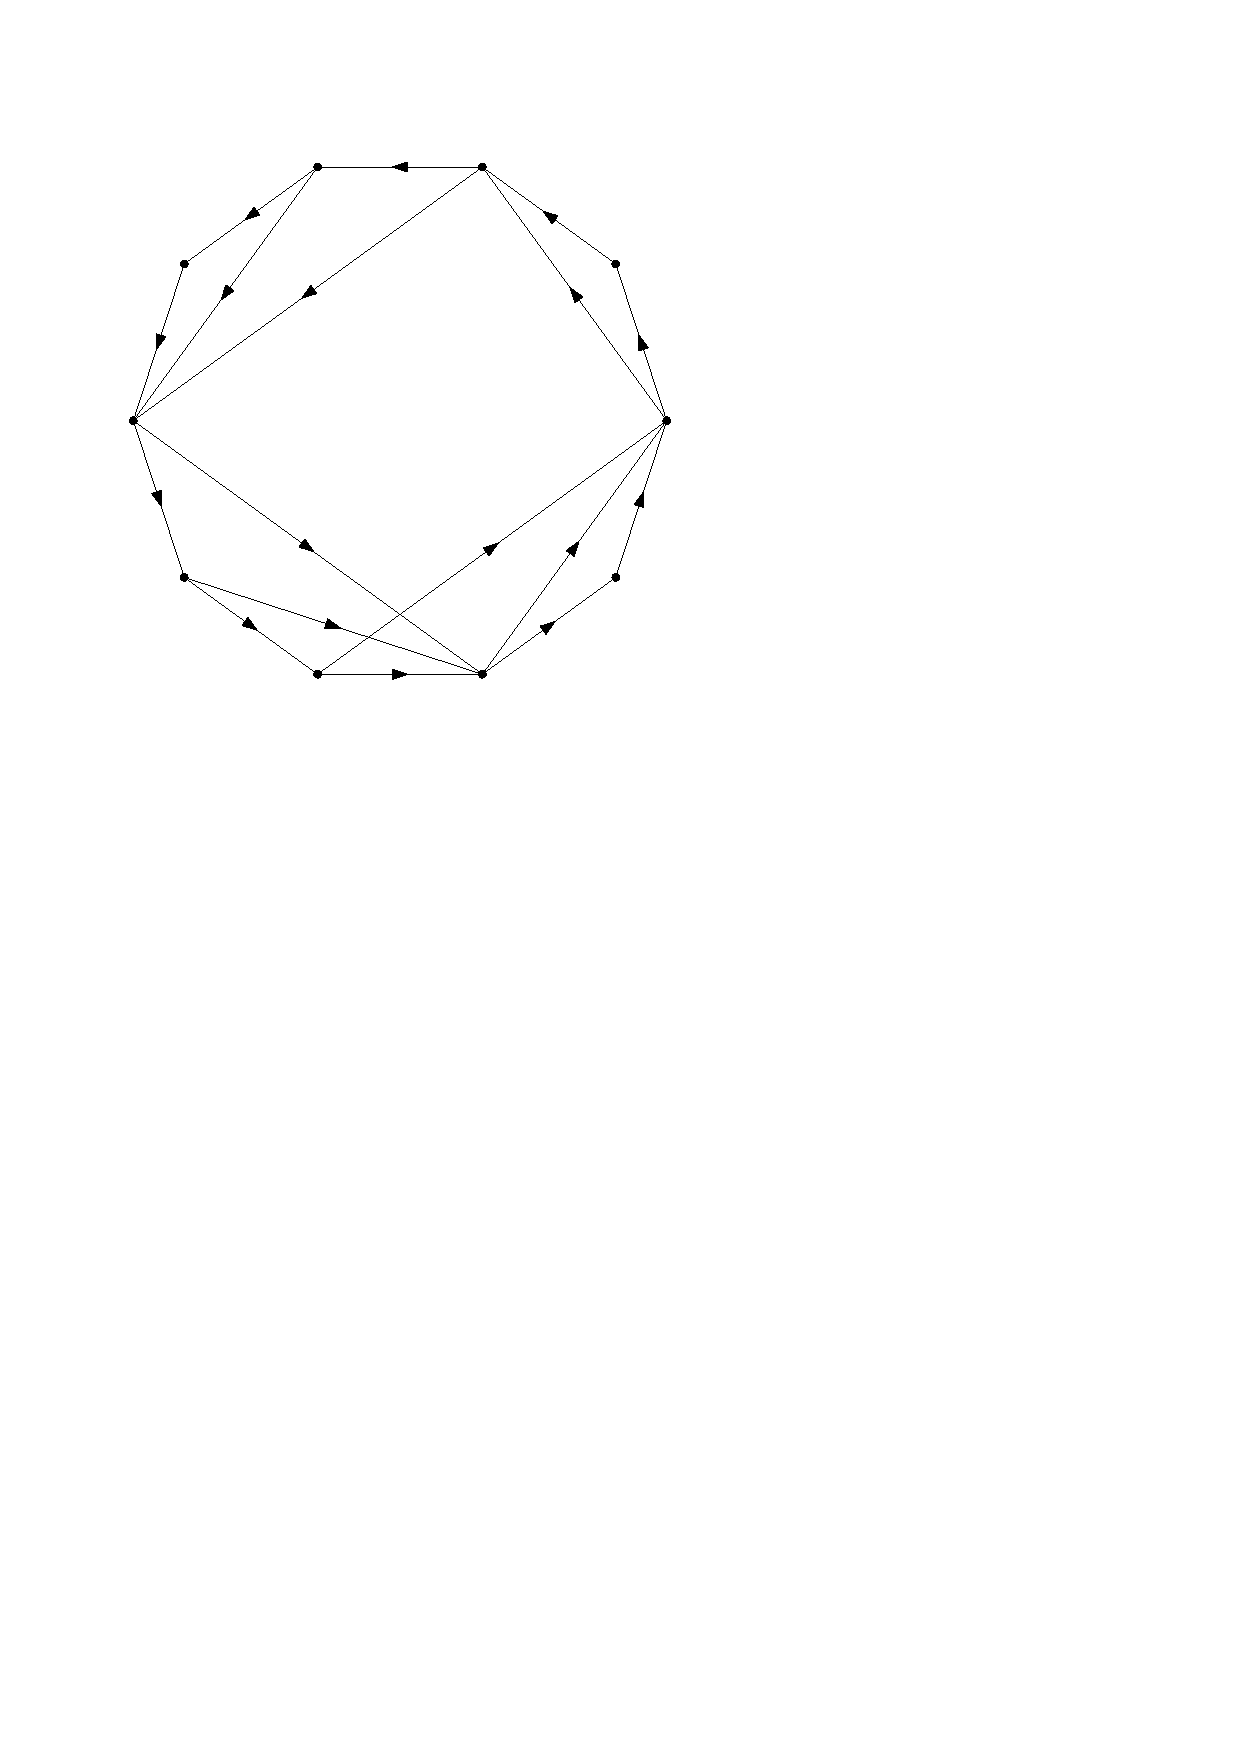
\includegraphics[scale=0.6]{Images/inround}}
\only<3>{

\textbf{Proof :}

\centering
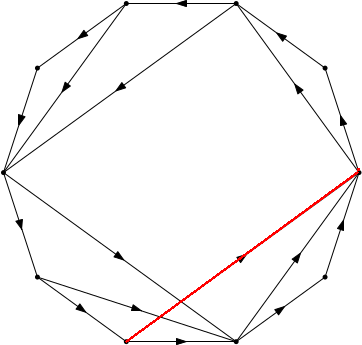
\includegraphics[scale=0.6]{Images/inround_colored}}

\only<4>{

\begin{theorem}
For any in-round oriented graph $G$ and vertex $v$, $G$ admits a $2$-dicolouring where $x^{+} \cup \{x\}$ is monochromatic.
\end{theorem}
}



\end{frame}

\end{document}
